%%%%%%%%%%%%  modele.tex
% exemple d'utilisation de la classe 
% etisbeamer.cls
%%%%%%%%%%%%%%%%%%%%%%%%%%%%%%%%%%%%%%%%%%%%%%%%%

\documentclass[miniframe]{marcelbeamer}
%\documentclass[handout]{etisbeamer}
%%%%%%%%%%%%% option de la classe etisbeamer.cls
% toutes les options standards de la classe beamer
% le type d'en-tete pour l'appel des sections : 
%  - default : currentsection | currentsubsection
%  - miniframe : sections + puces
%  - tree : sections + currentsubsection
%  - split : sections + subsections
%%%%%%%%%%%%%%%%%%%%%%%%%%%%%%%%%%%%%%%%%%%%%%%%%%

%%%%%%%%%%%%% appel des packages
\usepackage[english]{babel}
\usepackage{epsfig}
\usepackage[T1]{fontenc}
\usepackage[utf8]{inputenc}
\usepackage{lmodern} 
\usepackage{times}
\usepackage{multirow}
\usepackage{animate}
\usepackage{hyperref}
\usepackage{movie15}
\usepackage{wasysym}
\usepackage[squaren, Gray, cdot]{SIunits}

\usepackage{tabularx}
\newcolumntype{L}[1]{>{\raggedright\let\newline\\\arraybackslash\hspace{0pt}}m{#1}}
\newcolumntype{C}[1]{>{\centering\let\newline\\\arraybackslash\hspace{0pt}}m{#1}}
\newcolumntype{R}[1]{>{\raggedleft\let\newline\\\arraybackslash\hspace{0pt}}m{#1}}

\newcommand{\backupbegin}{
	\newcounter{framenumberappendix}
	\setcounter{framenumberappendix}{\value{framenumber}}
}
\newcommand{\backupend}{
	\addtocounter{framenumberappendix}{-\value{framenumber}}
	\addtocounter{framenumber}{\value{framenumberappendix}} 
}

%\usepackage{enumitem}

%%%%%%%%%%%%%%%%%%%%%%%%%%%%%%%%%%%%%%%%%%%%%%%%%%
%\newlist{fleche}{itemize}{1}
%\setlist[fleche]{label=$\rightarrow$,font=\color{blue}}


%\newcommand{\smiley}{\tikz[baseline=-0.75ex,black]{
%		    \draw circle (2mm);
%			\node[fill,circle,inner sep=0.5pt] (left eye) at (135:0.8mm) {};
%			\node[fill,circle,inner sep=0.5pt] (right eye) at (45:0.8mm) {};
%			\draw (-145:0.9mm) arc (-120:-60:1.5mm);
%			    }
%			}

\newcommand{\orto}{^{\circ}}

%%%%%%%%%%%%% appel du plan a chaque subsection
%% en 1 colonne

%\AtBeginSection[]{
%	\frame{%<handout:0>{
%	\frametitle{Plan}
%  \begin{columns}[t]
%  \begin{column}{0.5\linewidth}
%  \tableofcontents[sections={1-3}, currentsection,subsectionstyle=show/show/shaded]
%  \end{column}
%  \begin{column}{0.5\linewidth}
%  \tableofcontents[sections={4-6}, currentsection,subsectionstyle=show/show/shaded]
%  \end{column}
%  \end{columns}
%  }
%}

%% ou en 2 colonnes s'il y a trop de sections
    
%\AtBeginSubsection[]{
%	\frame{%<handout:0>{
%	\frametitle{Summary}
%  \begin{columns}[t]
%  \begin{column}{0.5\linewidth}
%  \tableofcontents[sections={1-6},currentsection, subsectionstyle=show/shaded/hide]
%  \end{column}
%  \begin{column}{0.5\linewidth}
%  \tableofcontents[sections={7-12},currentsection,subsectionstyle=show/shaded/hide]
%  \end{column}
%  \end{columns}
%  }
%}	
%%%%%%%%%%%%%%%%%%%%%%%%%%%%%%%%%%%%%%%%%%%%%%%%%%	

%%%%%%%%%%%%% Pour supprimer les symboles de navigation
\setbeamertemplate{navigation symbols}{}
%%%%%%%%%%%%%%%%%%%%%%%%%%%%%%%%%%%%%%%%%%%%%%%%%%

%%%%%%%%%%%%% Personnalisation des theoremes
\newtheorem{theoreme}{Th\'eor\`eme}
\newtheorem{preuve}{D\'emonstration}
\newtheorem{define}{D\'efinition}
%%%%%%%%%%%%%%%%%%%%%%%%%%%%%%%%%%%%%%%%%%%%%%%%%%	
		
%%%%%%%%%%%%%% Infos personnelles au document	
%\title[Auto-organisation matérielle]{Les effets de l’environnement sur le développement
%et l'organisation d'architectures de traitement matériel auto-organisées}
%%\subtitle{Première année de thèse}
%\author[L.Fiack]{Laurent Fiack\\\tiny{\\Thèse dirigée par Benoît Miramond}}
%%\email{}
%\institute[ETIS]{\textit{ETIS / ENSEA - Universit\'e de Cergy-Pontoise - CNRS UMR 8051 \\
%F-95000 Cergy-Pontoise Cedex, France}\\\\\textup{Financement :} Communauté d'Agglomération de Cergy-Pontoise}
%\date[2 décembre 2015]{}%\today]{}
%\logo{}%\includegraphics[height=0.1\textheight]{image}\hspace{1em}
%%%%%%%%%%%%%%%%%%%%%%%%%%%%%%%%%%%%%%%%%%%%%%%%%%%

%%%%%%%%%%%%% Infos personnelles au document	
\title[uC-RT]{Architecture du contrôleur temps-réel}
\subtitle{A$^3$: Du besoin à l'architecture}
\author[L. Fiack]{Laurent Fiack}
%\email{example@email.com}
\institute[MARCEL]{\textit{MARCEL - Address}}
\date[\today]{}
%\logo{}%\includegraphics[height=0.1\textheight]{image}\hspace{1em}
%%%%%%%%%%%%%%%%%%%%%%%%%%%%%%%%%%%%%%%%%%%%%%%%%%

\newcommand{\figpath}{figures/}

\begin{document}

%%%%%%%%%%%%% Background des slides	
\usebackgroundtemplate{}
%% cet option permet d'ins\'erer une image en fond-ecran
%% la commande \usebackgroundtemplate{} permet de
%% supprimer le fond a partir du moment ou il est 
%% appele
%%%%%%%%%%%%%%%%%%%%%%%%%%%%%%%%%%%%%%%%%%%%%%%%%%	

%%%%%%%%%%%%% frame title
\frame{\titlepage}
\usebackgroundtemplate{}
%\logo{}
%\logoheader{taille}{emplacement-image}
%% on supprime les logos des autres frames		
%%%%%%%%%%%%%%%%%%%%%%%%%%%%%%%%%%%%%%%%%%%%%%%%%%
%\frame{
%	\textcolor{blue1}{
%	\begin{tabular}{lllll}
%		Rapporteur  &:&B. Granado &-&LiP6\tabularnewline
%		Rapporteur &:&M. Paindavoine &-&LEAD\tabularnewline
%		Examinateur &:&S. Viollet &-&ISM\tabularnewline
%		Examinateur &:&N. Cuperlier &-&ETIS\tabularnewline
%		Examinateur &:&A. Upegui &-&InIT\tabularnewline
%		Directeur   &:&B. Miramond &-&LEAT\tabularnewline
%	\end{tabular}}
%}

\section[Architecture uC-RT]{Architecture du contrôleur temps-réel}
\subsection{Architecture uC-RT}
\frame{
	\frametitle{Robot mobile modulaire ?}

	\centering
	\begin{tabular}{l | p{65mm}}
		Fonction & Solution envisagée \\
		\hline \\ \pause
		Motorisation & Deux roues motrices indépendantes \\ \pause
		Évitement & Capteurs US/IR, Bumpers \\ \pause
		Alimentation & Batterie, BMS, Recharge \\ \pause
		Modularité & Interfaces, Programmabilité \\\\ \pause
		Vision & Caméra \\\\ \pause
		Prise de décision & Architecture de calcul \\\\
	\end{tabular}
}

\frame{
	\frametitle{Découpage fonctionnel}
	\centering
	\begin{tabular}{l | p{65mm}}
		Fonction & Architecture \\
		\hline \\ \pause
		Asservissements & Microcontrôleur temps-réel \\
		Odométrie & \\
		Alimentation (BMS) & \\
		Évitement & \\\\ \pause
		Servomoteurs & \\
		Interfaces & \\\\ \pause
		Vision & Microprocesseur programmable\\
		Learning & Calcul haute performance\\ 
	\end{tabular}
}

\frame{
	\frametitle{Découpage fonctionnel}
	\centering
	\includegraphics[width=0.6\linewidth]{figures/functions_rt}
}

\frame{
	\frametitle{Architecture de calcul}
	\centering
	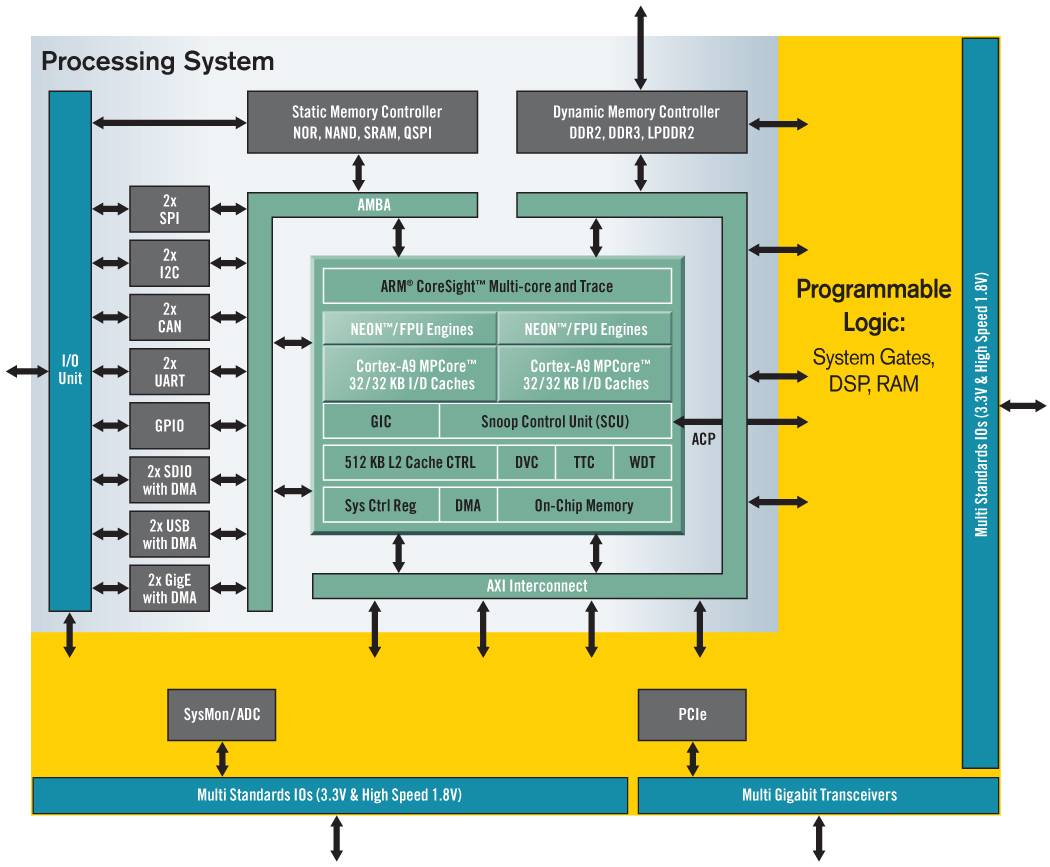
\includegraphics[width=0.7\linewidth]{figures/zynq_blockdiagram.jpg}
}

\frame{
	\frametitle{Architecture de calcul}
	\centering
	\includegraphics[width=0.8\linewidth]{figures/zynq_inside}
}

\frame{
	\frametitle{Architecture uC-RT}
	\begin{minipage}[b]{0.6\linewidth}
		\centering
		\includegraphics[width=\linewidth]{figures/uc-rt}
		\begin{block}{Périphériques}
			\begin{itemize}
				\item Instanciation dans \texttt{top.vhd}
				\item "\texttt{system.h}"
			\end{itemize}
		\end{block}
	\end{minipage}
	\hfill
	\begin{minipage}[b]{0.35\linewidth}
		\begin{block}{Memory Map}
			\begin{itemize}
				\item @0 ... @P
				\item @P ... @P+D
				\item @FFFF-C ... @C
			\end{itemize}
		\end{block}
		\begin{block}{Impact sur...}
			\begin{itemize}
				\item \texttt{omsp\_defines.v}
				\item \texttt{link.ld}
			\end{itemize}
		\end{block}
	\end{minipage}
}

\frame{
	\frametitle{DMA}
	\begin{minipage}[b]{0.6\linewidth}
		\centering
		\includegraphics[width=\linewidth]{figures/uc-rt_dma}
	\end{minipage}
	\hfill
	\begin{minipage}[b]{0.35\linewidth}
	\end{minipage}

}

\frame{
	\frametitle{Organisation Code ?}
	\centering
	???
}

%%\section[Short Title 1]{Long Title 1}
%%\subsection{Subsection 1}
%%\frame{
%%	\frametitle{Subsection 1.1}
%%}
%%
%%\frame{
%%	\frametitle{Subsection 1.2}
%%}
%%
%%\subsection{Subsection 2}
%%\frame{
%%	\frametitle{Subsection 2.1}
%%}
%%
%%\frame{
%%	\frametitle{Subsection 2.2}
%%}
%%
%%\section[Short Title 2]{Long Title 2}
%%\subsection{Subsection 1}
%%\frame{
%%	\frametitle{Subsection 1.1}
%%}
%%
%%\frame{
%%	\frametitle{Subsection 1.2}
%%}
%%
%%\subsection{Subsection 2}
%%\frame{
%%	\frametitle{Subsection 2.1}
%%}
%%
%%\frame{
%%	\frametitle{Subsection 2.2}
%%}
%%
%%\appendix
%%\backupbegin
%%
%%\frame{
%%	\frametitle{Backup 1}
%%}
%%
%%\frame{
%%	\frametitle{Backup 2}
%%}
%%
%%\backupend
\end{document}
